\section{Orbit Measurements}
\subsection{Beam position and intensity}
\label{sec.02_OrbitMeas}

Orbit was measured with several types of devices, 
see Section~\ref{sec:BI:BeamPosition} for details.
All the BPMs were interfaced with the CERN universal readout system for this kind of devices called XenericSampler.
Thanks to it, the generic displays developed for the PS Complex could be used
both for orbit and for showing the traces along the beam pulse. 
%Additionally to providing traces for beam intensity and position XenericSampler calculated mean positions 
%intervals in of 280~ns, corresponding to the CR time of flight.
Around 2006, when the architecture of the control system changed from GM to FESA
and the CERN control system application framework moved to Java,
dedicated Java applications were developed. 
They could save orbits as references, which was an important feature to detect orbit changes,
to correct the orbit back to the reference and to perform quick checks during the machine setup.
Also orbit for different parts of the pulse and their differences could displayed,
which was crucial for the beam recombination setup and monitoring. 

The round aperture BPMs were very reliable and yielded 0.1~mm resolution with a good linearity.
On the other hand, BPIs displayed several issues.
Because CTF3 was constructed in stages it was possible to correct the observed imperfections
in the devices fabricated for the following stage. Therefore, each of the machine sections
had slightly different BPIs.
The first version installed in the CT line and in the DL
showed large droops, which was varying with the beam position and charge.
A correction was eventually implemented in the read-out software.
For each of the four electrodes parameters of the exponential decay were
evaluated and subtracted from the digitized signal. 
Next versions installed in the remaining part of the machine had this effect reduced at different levels. 
Still, for long acquisitions of the beam circulating in the CR 
it was clearly visible, see Figure~\ref{fig:bpi_charging_up}. 
This is to be compared to a BPM, as seen in figure~\ref{fig:bpm_not_charging_up}, 
where this effect is not present in the position signal. 
Additionally, it could not be software corrected because 
for newer versions the sum and difference signals of the electrodes
were evaluated with a local amplifier
so only 3 cables were connected to the read-out electronics. 


\begin{figure}
\begin{center}
% 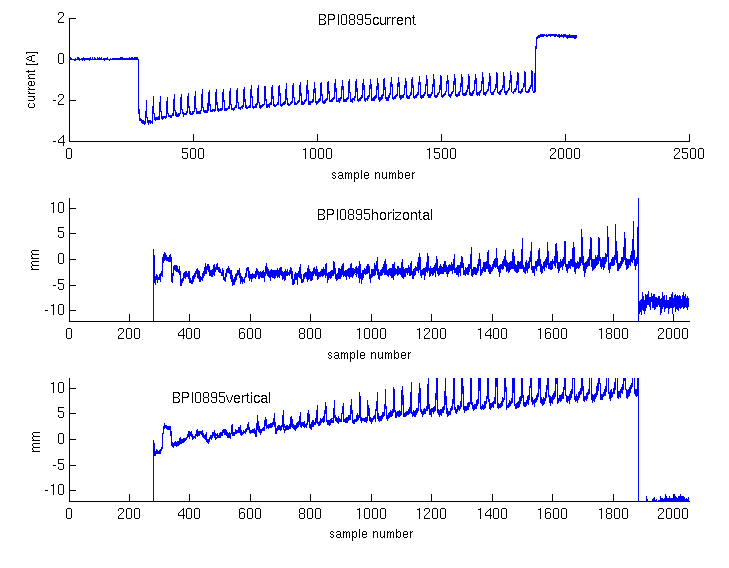
\includegraphics[width=1\linewidth,natwidth=729,natheight=568]{BPI0895.png}
 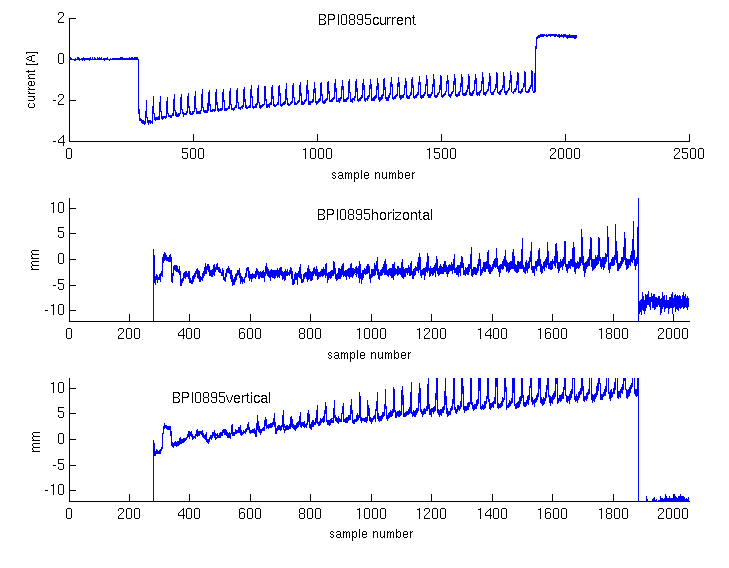
\includegraphics[width=0.8\linewidth]{BPI0895.png}
 \caption{Example reading of a BPI in the Combiner Ring for a circulating beam.}
\label{fig:bpi_charging_up}
\end{center}
\end{figure}

\begin{figure}
\begin{center}
 %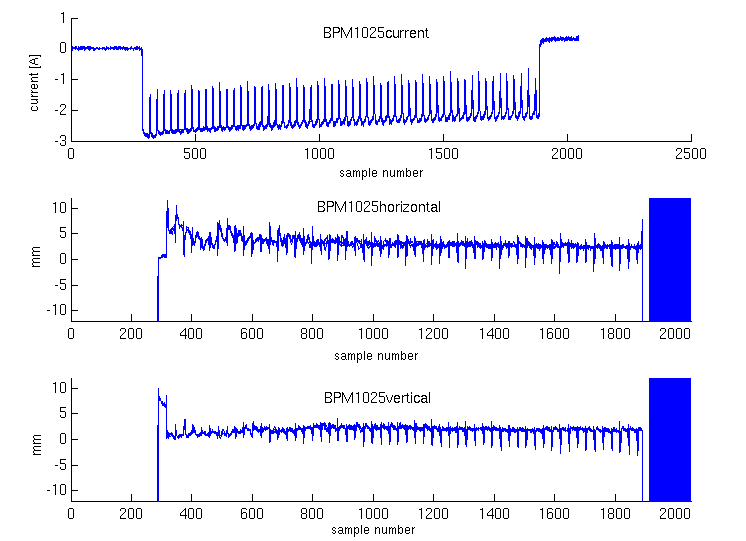
\includegraphics[width=1\linewidth,natwidth=746,natheight=541]{BPM1025.png}
 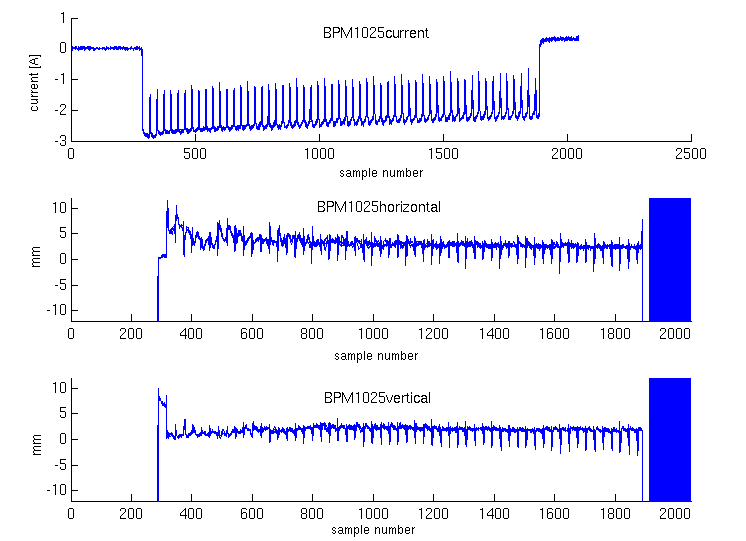
\includegraphics[width=0.8\linewidth]{BPM1025.png}
 \caption{Example reading of a BPM in the Combiner Ring for a circulating beam.}
\label{fig:bpm_not_charging_up}
\end{center}
\end{figure}


Another important issue was related to nonlinearities. In TL1 it was observed that 
changing the bunch frequency from 3 to 1.5~GHz made the BPM readout completely different, 
while it was the same in the sections before and after. 
Dedicated beam measurements were made to quantify the effect and 
the issue was confirmed, however, it was never understood and resolved. 
For this reason orbit optimization and studies in TL1 were done only with 3~GHz beam.
For 1.5~GHz beam TL1 BPMs were not considered.
For all BPIs the beam current measurement was very nonlinear and 
at 28~A they overestimated the current by 
circa 15\% while at low current they perfectly agreed with other BPMs. 
On top of that, the nonlinearity was different for each device.
This is the reason for the orbit displays showing often uneven beam current pattern along the machine. 


